%%%%%%%%%%%%%%%%%%%%%%%%%%%%%%%%%%%%%%%%%
% Beamer Presentation
% LaTeX Template
% Version 1.0 (10/11/12)
%
% This template has been downloaded from:
% http://www.LaTeXTemplates.com
%
% License:
% CC BY-NC-SA 3.0 (http://creativecommons.org/licenses/by-nc-sa/3.0/)
%
%%%%%%%%%%%%%%%%%%%%%%%%%%%%%%%%%%%%%%%%%

\documentclass[t]{beamer}

\usepackage[english]{babel}
\usepackage[utf8]{inputenc}
\usepackage{hyperref}
\usepackage{verbatim}
\usepackage{listings}

%----------------------------------------------------------------------------------------
%	PACKAGES AND THEMES
%----------------------------------------------------------------------------------------

\mode<presentation> {

% The Beamer class comes with a number of default slide themes
% which change the colors and layouts of slides. Below this is a list
% of all the themes, uncomment each in turn to see what they look like.

%\usetheme{default}
%\usetheme{AnnArbor}
%\usetheme{Antibes}
%\usetheme{Bergen}
%\usetheme{Berkeley}
%\usetheme{Berlin}
%\usetheme{Boadilla}
%\usetheme{CambridgeUS}
%\usetheme{Copenhagen}
%\usetheme{Darmstadt}
%\usetheme{Dresden}
%\usetheme{Frankfurt}
%\usetheme{Goettingen}
%\usetheme{Hannover}
%\usetheme{Ilmenau}
%\usetheme{JuanLesPins}
%\usetheme{Luebeck}
%\usetheme{Madrid}
%\usetheme{Malmoe}
%\usetheme{Marburg}
%\usetheme{Montpellier}
%\usetheme{PaloAlto}
%\usetheme{Pittsburgh}
%\usetheme{Rochester}
%\usetheme{Singapore}
%\usetheme{Szeged}
\usetheme{Warsaw}

% As well as themes, the Beamer class has a number of color themes
% for any slide theme. Uncomment each of these in turn to see how it
% changes the colors of your current slide theme.

%\usecolortheme{albatross}
%\usecolortheme{beaver}
%\usecolortheme{beetle}
%\usecolortheme{crane}
%\usecolortheme{dolphin}
%\usecolortheme{dove}
%\usecolortheme{fly}
%\usecolortheme{lily}
%\usecolortheme{orchid}
%\usecolortheme{rose}
\usecolortheme{seagull}
%\usecolortheme{seahorse}
%\usecolortheme{whale}
%\usecolortheme{wolverine}

\usefonttheme{structuresmallcapsserif}

%\setbeamertemplate{footline} % To remove the footer line in all slides uncomment this line
%\setbeamertemplate{footline}[page number] % To replace the footer line in all slides with a simple slide count uncomment this line

%\setbeamertemplate{navigation symbols}{} % To remove the navigation symbols from the bottom of all slides uncomment this line
}


\usepackage{graphicx} % Allows including images
\usepackage{booktabs} % Allows the use of \toprule, \midrule and \bottomrule in tables



\lstdefinestyle{cpp}{
  language=C++,
  basicstyle=\ttfamily\footnotesize,  % Use small true type font
  showstringspaces=false,                 % Don't put marks in string spaces
  tabsize=2,                              % 5 spaces per tab
  escapeinside={@}{@},                % for invisible labels
  breaklines=true,
  breakatwhitespace=true,
  emptylines=1,
  texcl=true,
  escapechar=@,
  mathescape=true,
  xleftmargin=2.5ex,
  keywordstyle=[1]\color{blue},
  % keywordstyle=[2]\color{red},
	% stringstyle=\color{red},
	% commentstyle=\color{green},
	% morekeywords=[1]{pop_front}
	% morekeywords=[2]{parent,child}
}

\usepackage{wrapfig}
\author[]{Kevin Wallimann \quad Johannes Baum \quad Matthias Untergassmair}

%----------------------------------------------------------------------------------------
%	TITLE PAGE
%----------------------------------------------------------------------------------------

\title[Topological Sorting]{Parallel Topological Sorting} % The short title appears at the bottom of every slide, the full title is only on the title page
\subtitle{Design of High Performance Computing, Fall 2015}

\institute[ETHZ]{ ETH Zürich }
%\date{\today} % Date, can be changed to a custom date
\date{December 14, 2015}
	\begin{document}

\begin{frame}
\titlepage % Print the title page as the first slide
\end{frame}

%----------------------------------------------------------------------------------------
%	PRESENTATION SLIDES
%----------------------------------------------------------------------------------------

%------------------------------------------------
\section{Overview}
%------------------------------------------------


\begin{frame}
\frametitle{Overview}

\begin{itemize}
\item DAG defines partial order
\item Topological sorting defines one total order on a DAG
\item Parallel algorithm: finds one topological sorting of a given DAG
\end{itemize}

\begin{figure}[!hbp]
 
  \begin{tikzpicture}[->,>=stealth',auto,node distance=1cm,
                    thick,main
                    node/.style={circle,draw,font=\sffamily\scriptsize},text node/.style={draw=none,font=\sffamily\tiny}]

  \node[main node] (1) [draw=black!80,text=black!80] {1};
  \node[main node] (3) [right of=1, node distance=1.2cm]{3};
  \node[main node] (7) [below of=3, node distance=1.2cm] {7};
  \node[main node] (4) [left of=7, node distance=1.2cm] {4};
  \node[main node] (5) [below of=7, node distance=1.2cm] {5};
  \node[main node] (6) [left of=4, node distance=1.2cm] {6};
  \node[main node] (8) [left of=5, node distance=1.2cm] {8};
  \node[main node] (9) [below of=8, node distance=1.2cm] {9};
  \node[main node] (2) [left of=8, node distance=1.2cm] {2};
  
  \node[text node] (11) [below right of=1, node distance=0.5cm] {1};
  \node[text node] (31) [below right of=3, node distance=0.5cm] {2};
  \node[text node] (71) [below right of=7, node distance=0.5cm] {3};
  \node[text node] (41) [below right of=4, node distance=0.5cm] {4};
  \node[text node] (51) [below right of=5, node distance=0.5cm] {4};
  \node[text node] (61) [below left of=6, node distance=0.5cm] {5};
  \node[text node] (81) [below right of=8, node distance=0.5cm] {5};
  \node[text node] (91) [below right of=9, node distance=0.5cm] {1};
  \node[text node] (21) [below left of=2, node distance=0.5cm] {2};

  


  \path[every node/.style={font=\sffamily\small}]
    (1) edge (3)
    (3) edge (7)
    (7) edge (4)
    (4) edge (6)
    (7) edge (5)
    (5) edge (8)
    (8) edge (6)
    (9) edge (5)
    (9) edge (2)
    (2) edge (8)
    ;
\end{tikzpicture}

\begin{tikzpicture}[-,>=stealth',auto,node distance=0.85cm,minimum
height=0.85cm, minimum width=0.85cm,main
                    node/.style={rectangle,draw,font=\sffamily\footnotesize}]
                    
       
  \node[main node] (0) [minimum width=1.5cm, font=\bfseries\footnotesize]
  {Name}; \node[main node] (1) [right of=0, node distance=1.2cm] {1};
  \node[main node] (2) [right of=1] {9};
  \node[main node] (3) [right of=2] {2};
  \node[main node] (4) [right of=3] {3};
  \node[main node] (5) [right of=4] {7};
  \node[main node] (6) [right of=5] {4};
  \node[main node] (7) [right of=6] {5};
  \node[main node] (8) [right of=7] {8};
  \node[main node] (9) [right of=8] {6};

  \node[main node] (12) [minimum width=1.5cm, below of=0,
  font=\bfseries\footnotesize] {Value}; \node[main node] (13) [below of=1] {1};
  \node[main node] (14) [below of=2] {1};
  \node[main node] (15) [below of=3] {2};
  \node[main node] (16) [below of=4] {2};
  \node[main node] (17) [below of=5] {3};
  \node[main node] (18) [below of=6] {4};
  \node[main node] (19) [below of=7] {4};
  \node[main node] (20) [below of=8] {5};
  \node[main node] (21) [below of=9] {5};

  


\end{tikzpicture}


\end{figure}

\end{frame}

%------------------------------------------------
\section{Difference to BFS}
%------------------------------------------------

\begin{frame}
\frametitle{Difference to BFS}

\begin{itemize}
\item BFS visits every node
\item Topological sorting algorithm needs to visit every edge
\end{itemize}

Example:

\begin{figure}[!hbp]
 
  \begin{tikzpicture}[->,>=stealth',auto,node distance=1cm,
                    thick,main
                    node/.style={circle,draw,font=\sffamily\scriptsize},text node/.style={draw=none,font=\sffamily\tiny}]

  \node[main node] (1) [draw=black!80,text=black!80] {A};
  \node[main node] (2) [below right of=1, node distance=1.2cm]{B};
  \node[main node] (3) [below of=1, node distance=1.2cm] {C};
  

  \path[every node/.style={font=\sffamily\small}]
    (1) edge (2)
    (2) edge (3)
    (1) edge (3)
    ;
\end{tikzpicture}

\end{figure}

Consider order A,C,B
$\rightarrow$ valid in BFS, invalid in topological sorting

\end{frame}

%------------------------------------------------
\section{Input graphs}
%------------------------------------------------
\begin{frame}
\frametitle{Random graph}

\begin{columns}[c]
 \column{0.29\textwidth}
 \begin{itemize}
  \item Parameter: Average node degree
 \end{itemize}

 \column{0.7\textwidth}
 \begin{figure}[!hbp]
    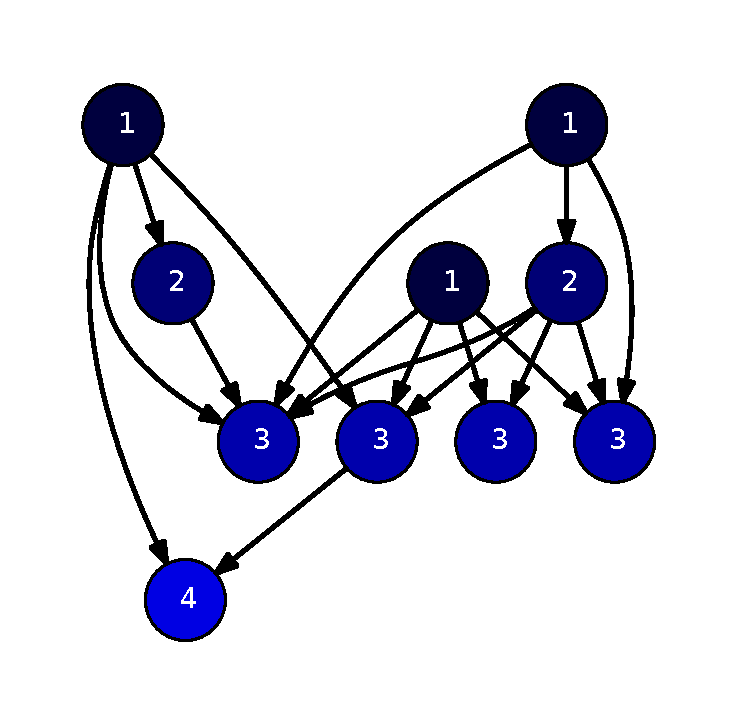
\includegraphics[height=0.7\textheight]{img/random_lin10.pdf}
 \end{figure}
\end{columns}

\end{frame}

\begin{frame}
\frametitle{Software dependency graph}

\begin{columns}[c]
 \column{0.29\textwidth}
 \begin{tabular}{p{1cm}p{1cm}p{1.5cm}}
  Nodes    & Edges   & Degree (Median)\\\hline
  100'000  & 266'680 & 2\\
  10'000   & 27'416  & 2
 \end{tabular}
 \column{0.7\textwidth}
 \begin{figure}[!hbp]
    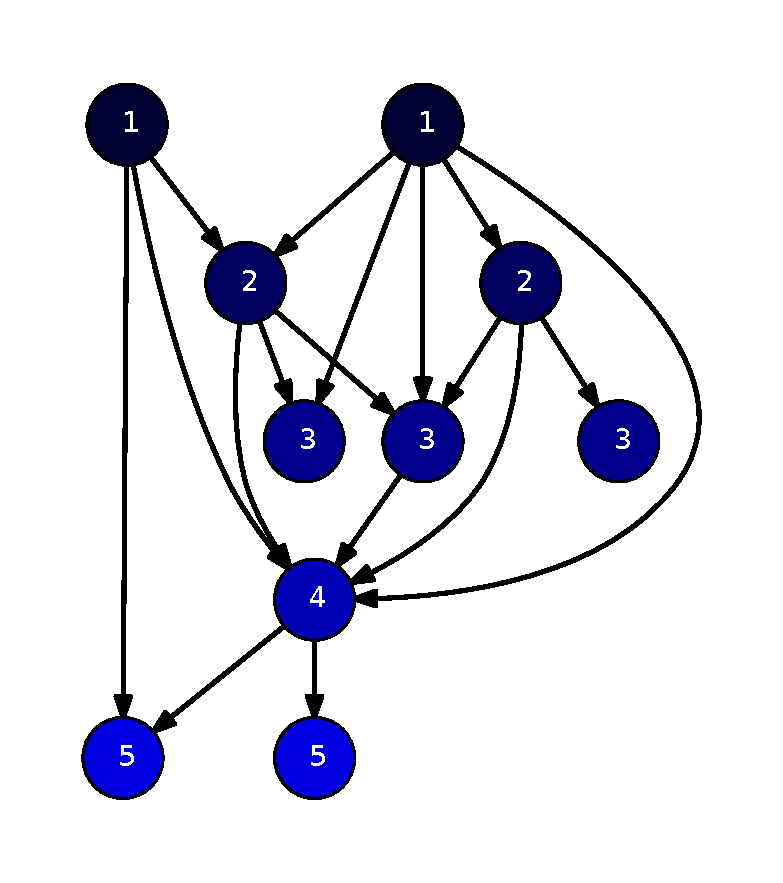
\includegraphics[height=0.7\textheight]{img/software10.pdf}
 \end{figure}
\end{columns}
{\color{gray}\tiny Musco, V. et al. (2014) "A Generative Model of Software Dependency Graphs to Better Understand Software Evolution."}

\end{frame}


%------------------------------------------------
\section{Implementations}
%------------------------------------------------

\begin{frame}
\frametitle{Parallel algorithm (shared memory)}

\begin{columns}[c]
 \column{0.7\textwidth}
  \begin{enumerate}
    \item As a preparing step, initialize a counter for every child with the number of its parents.
    \item Distribute parent nodes over threads and process them in parallel.
    \item For every parent node, get a list of all child nodes and append the parent itself to solution ($\rightarrow$ \textbf{lock}).
    \item For every child of the parent, decrement its counter ($\rightarrow$ \textbf{lock}). Once the counter is zero, we can move on
    \item When all parents are processed ($\rightarrow$ \textbf{barrier}), distribute new nodes and repeat
  \end{enumerate}

 \column{0.3\textwidth}
  \begin{figure}[!ht]
    \begin{center}
      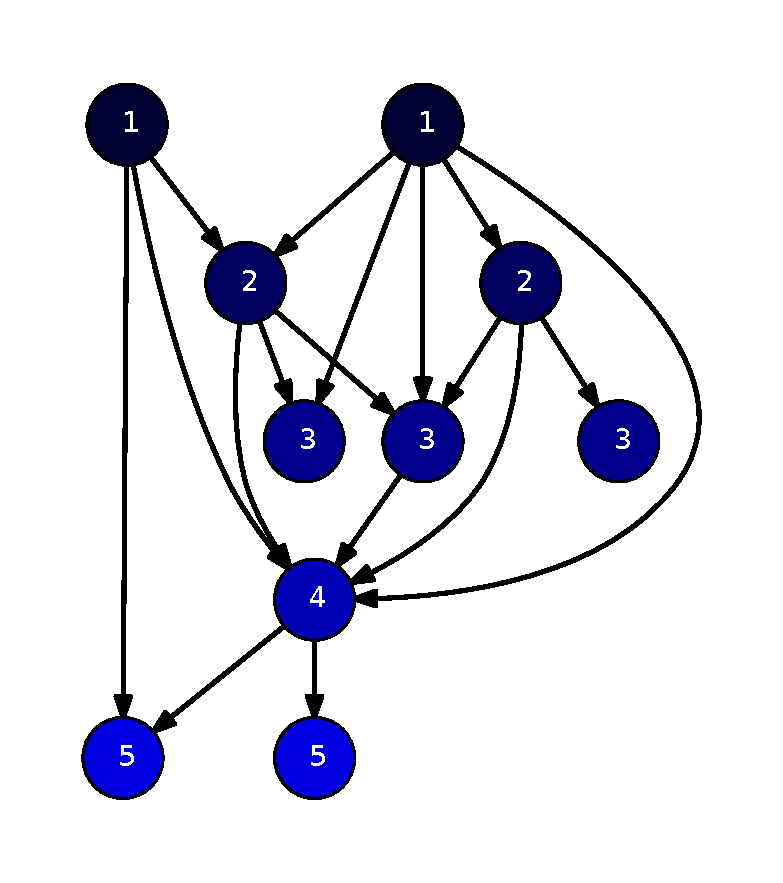
\includegraphics[width=\textwidth]{img/software10.pdf}
    \end{center}
  \end{figure}
\end{columns}

\end{frame}


\begin{frame}
 \frametitle{Local lists approach}
 \textbf{Idea:} perfect load balancing by redistributing nodes at every step
  \begin{itemize}
  \item Parent nodes stored in a global list.
  \item Distribution of parent nodes: \emph{scatter} the list among the threads. Each thread has now its local list.
  \item Add new nodes to the end of local list.
  \item When all parents were processed, \emph{gather} all local lists into the global list.
  \item Repeat until there are no parents left in the global list.
  \end{itemize}
  
\end{frame}

\begin{frame}
 \frametitle{Boolean array approach}
 \textbf{Idea:} minimizing memory access by using lookup table 
 \begin{itemize}
  \item Array of length $N$. 1 if node $i$ is a parent node, 0 otherwise.
  \item Distribution of parent nodes: Parallel for-loop through the array.
  \item Mark new parents by setting a 1 in a second array.
  \item When all parents were processed, swap arrays.
  \item Loop through the array until there are no new parents.
 \end{itemize}
 
\end{frame}

\begin{frame}[fragile]
 \frametitle{Optimistic counter check}
 \begin{itemize}
  \item Decrement shared counter
  \item Return true if counter is zero
 \end{itemize}
 \begin{lstlisting}[style=cpp]
  inline bool counterCheck() {
          bool lastone;
          #pragma omp critical
          {
            --parcount_;
            lastone = (parcount_ == 0);
          }
          return lastone;
  }
 \end{lstlisting}
\end{frame}

\begin{frame}[fragile]
 \frametitle{Optimistic counter check}
 \begin{itemize}
  \item Decrement shared counter
  \item Return true if counter is zero
 \end{itemize}
 \begin{lstlisting}[style=cpp]
  inline bool counterCheck() {
          #pragma omp atomic
          --parcount_;
          return (parcount_ == 0);
  }
 \end{lstlisting}
 \begin{itemize}
  \item Multiple threads could return true, although only one thread should do so.
 \end{itemize}
\end{frame}

\begin{frame}[fragile]
 \frametitle{Optimistic counter check}
  \begin{lstlisting}[style=cpp]
  inline bool counterCheck() {
          #pragma omp atomic
          --parcount_;
          return (parcount_ == 0);
  }
 \end{lstlisting}
 \begin{itemize}
  \item List based approach: Child is inserted multiple times to solution $\Rightarrow$ Wrong.
  \item Array approach: Multiple threads write 1 to the array $\Rightarrow$ Ok, doesn't matter.
 \end{itemize}
\end{frame}

%------------------------------------------------
\section{Architecture}
%------------------------------------------------
\begin{frame}
  \frametitle{Euler}
  \begin{itemize}
  \item Intel Xeon E5 on Euler cluster
  \item 2 processors per node
  \item 12 cores
  \item 30 MB shared last-level cache
  \item Software graph with around 1M nodes should fit into cache % TODO: Maybe it's a little odd to state this here
  \end{itemize}
\end{frame}

%------------------------------------------------
\section{Results}
%------------------------------------------------

\begin{frame}
\frametitle{Strong scaling software graph}
\begin{columns}[T]
 \column{0.5\textwidth}
  \bfseries{Local lists}
  \begin{figure}[!ht]
    \begin{center}
      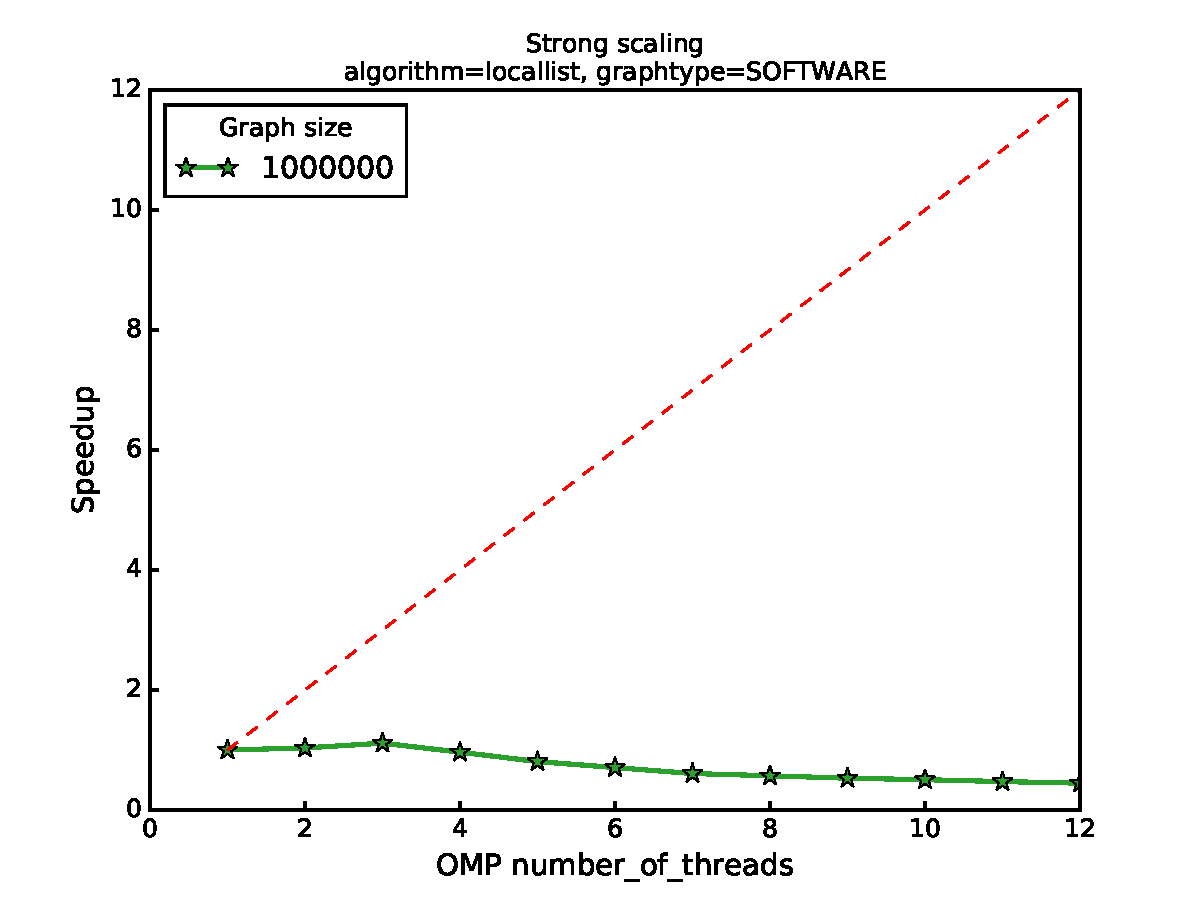
\includegraphics[width=\textwidth]{img/strongscaling_locallist_gtSOFTWARE_opt0.pdf}
    \end{center}
  \end{figure}
 \column{0.5\textwidth}
  \bfseries{Bool array}
  \begin{figure}[!ht]
    \begin{center}
      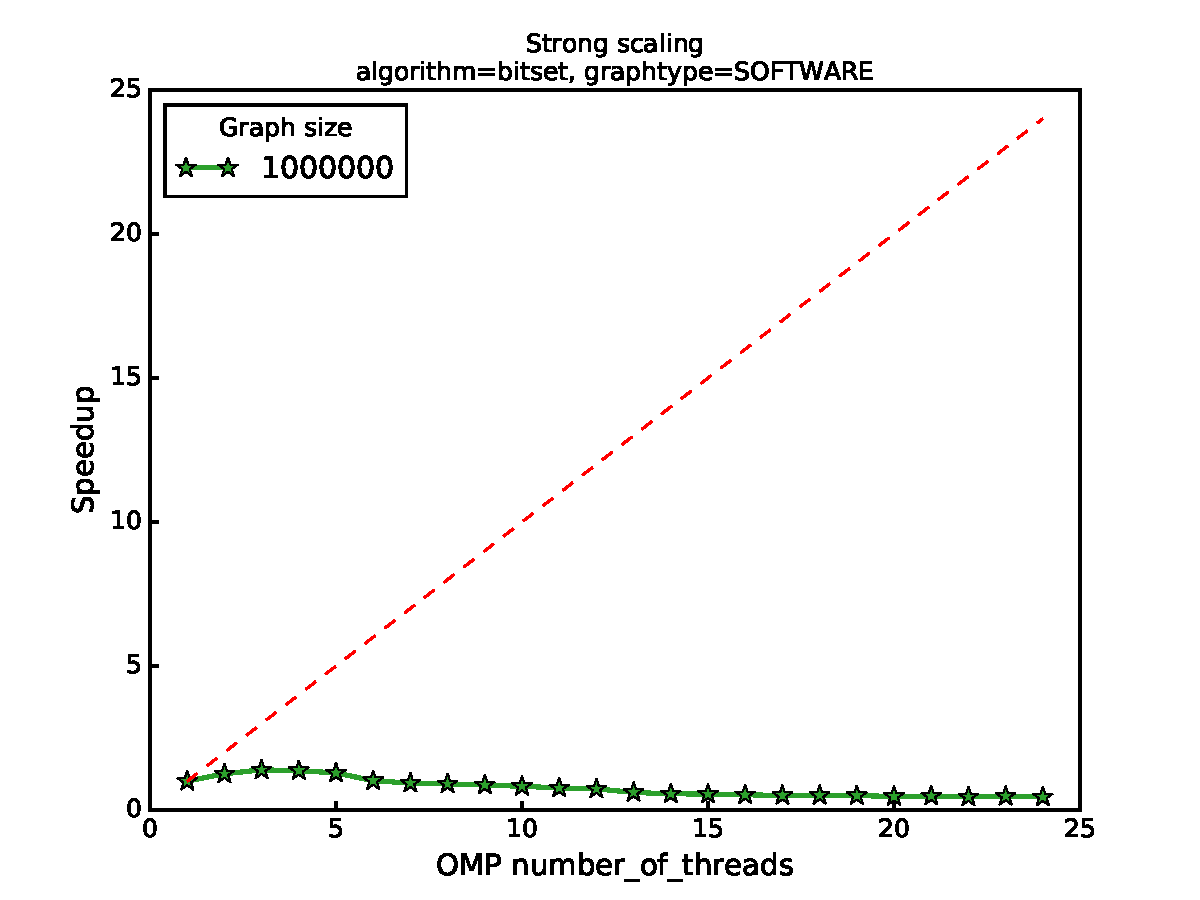
\includegraphics[width=\textwidth]{img/strongscaling_bitset_gtSOFTWARE_opt1.pdf}
    \end{center}
  \end{figure}  
\end{columns}

\begin{table}
\tiny
\begin{tabular}{lp{1cm}|p{1cm}|p{1cm}}
 {\bfseries Absolute runtimes on 1 core}  & serial  & bool array  & local list\\
                                          & 0.45 s  & 0.58 s      & 0.48 s
\end{tabular}
\end{table}

\end{frame}


\begin{frame}
\frametitle{Bool array \& random graph (node degree 30)}
\begin{columns}[T]
 \column{0.5\textwidth}
  \bfseries{Strong scaling}
  \begin{figure}[!ht]
    \begin{center}
      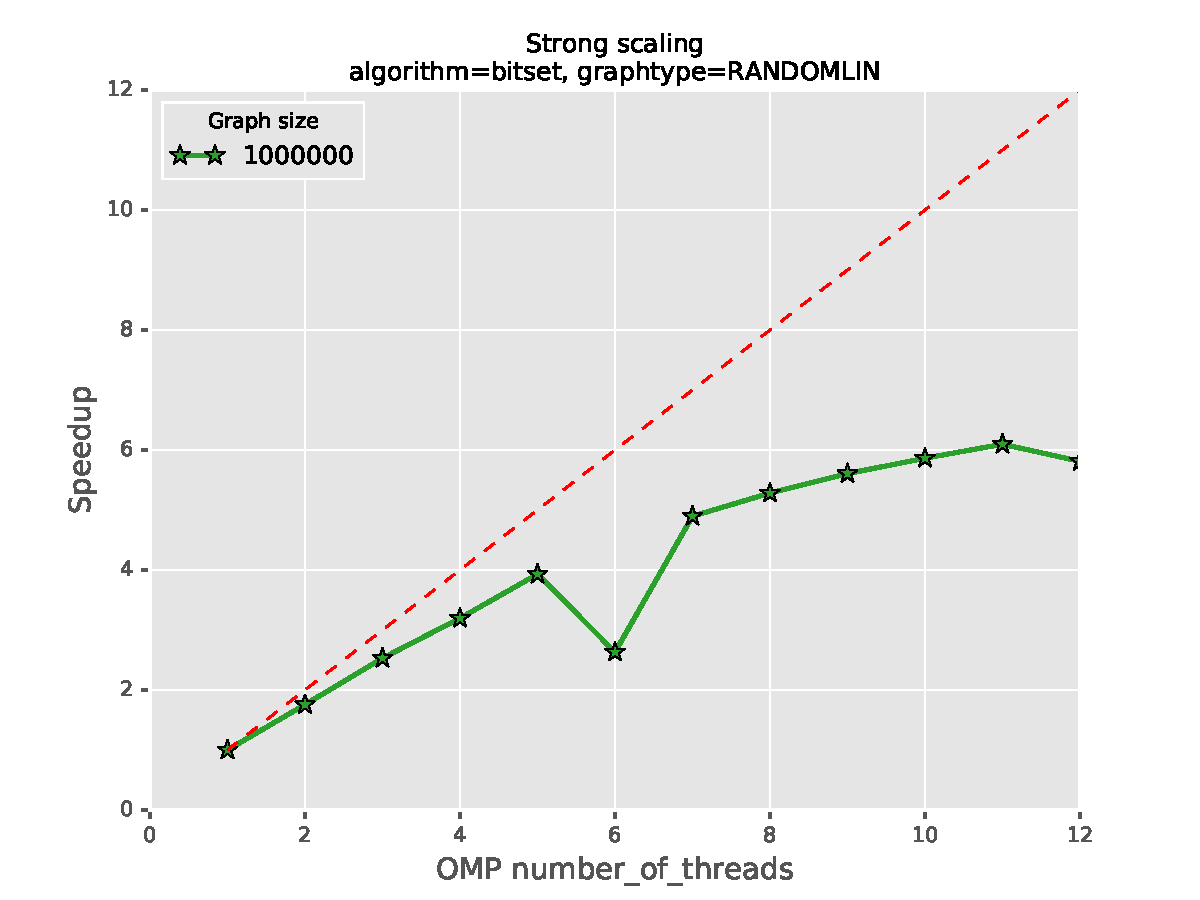
\includegraphics[width=\textwidth]{img/strongscaling_bitset_gtRANDOMLIN30_opt1.pdf}
    \end{center}
  \end{figure}
 \column{0.5\textwidth}
  \bfseries{Weak scaling}
  \begin{figure}[!ht]
    \begin{center}
      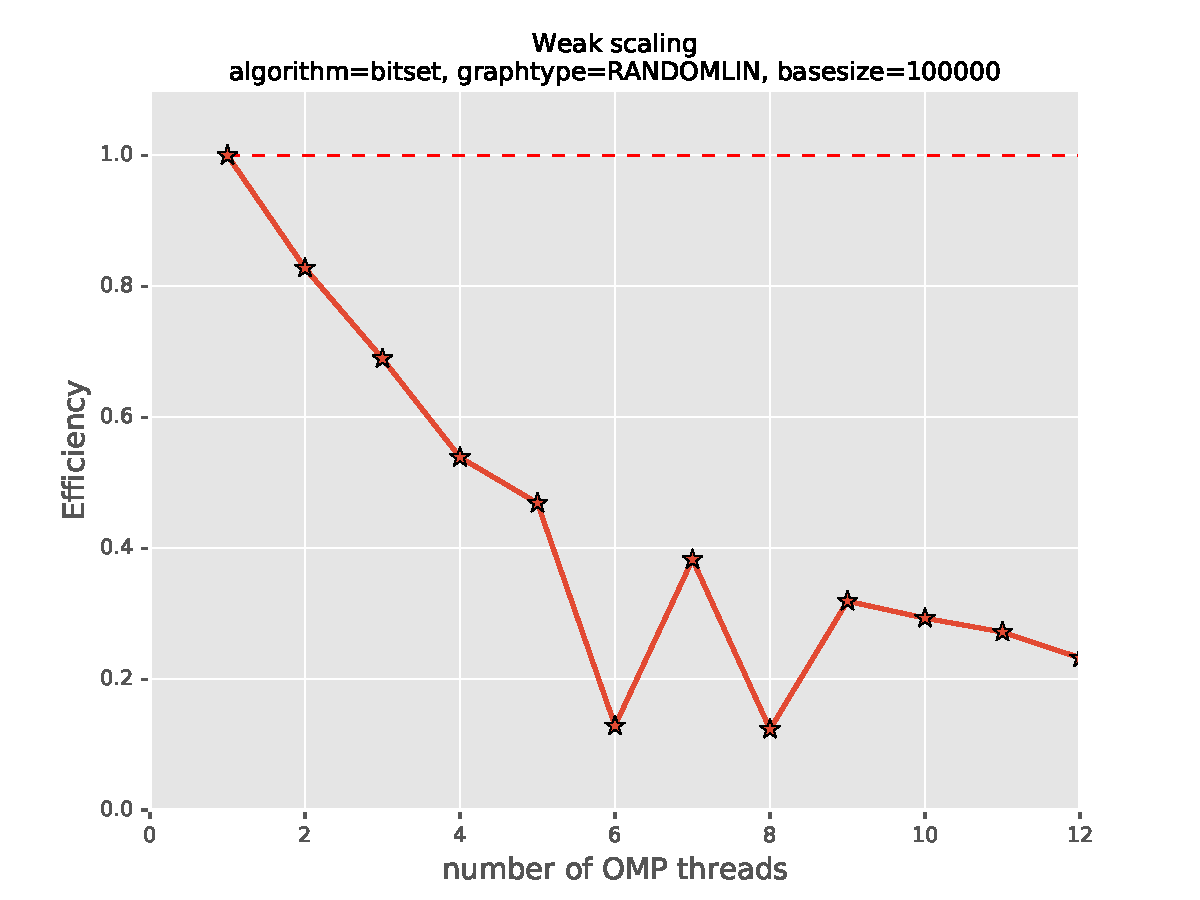
\includegraphics[width=\textwidth]{img/weakscaling_bitset_gtRANDOMLIN30_opt1.pdf}
    \end{center}
  \end{figure}  
\end{columns}

\begin{table}
\tiny
\begin{tabular}{lp{1cm}|p{1cm}}
 {\bfseries Absolute runtimes on 1 core}  & serial  & bool array \\
                                          & 2.76 s  & 3.51 s
\end{tabular}
\end{table}

\end{frame}

\begin{frame}
\frametitle{Optimistic counter check}
\begin{columns}[T]
 \column{0.5\textwidth}
  \bfseries{Optimistic}
  \begin{figure}[!ht]
    \begin{center}
      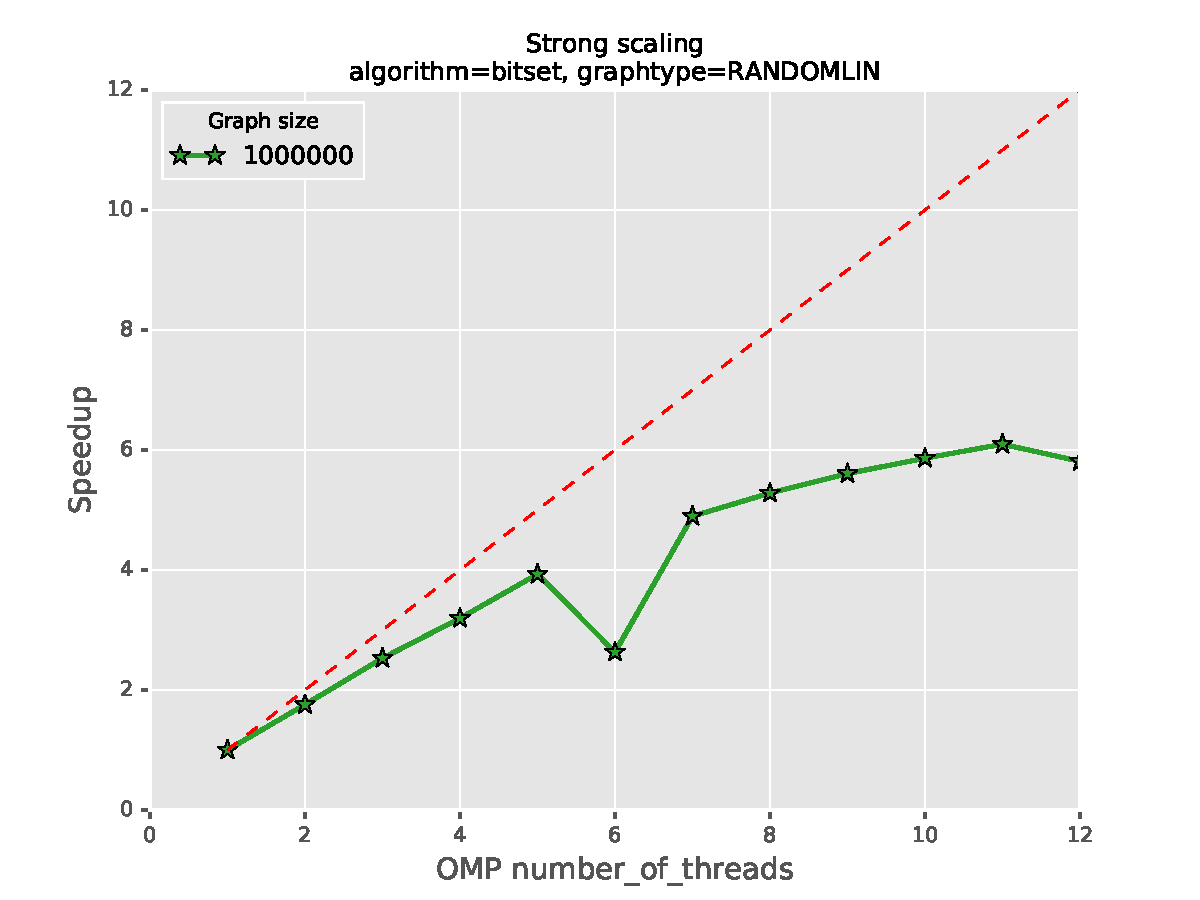
\includegraphics[width=\textwidth]{img/strongscaling_bitset_gtRANDOMLIN30_opt1.pdf}
    \end{center}
  \end{figure}
 \column{0.5\textwidth}
  \bfseries{Conventional}
  \begin{figure}[!ht]
    \begin{center}
      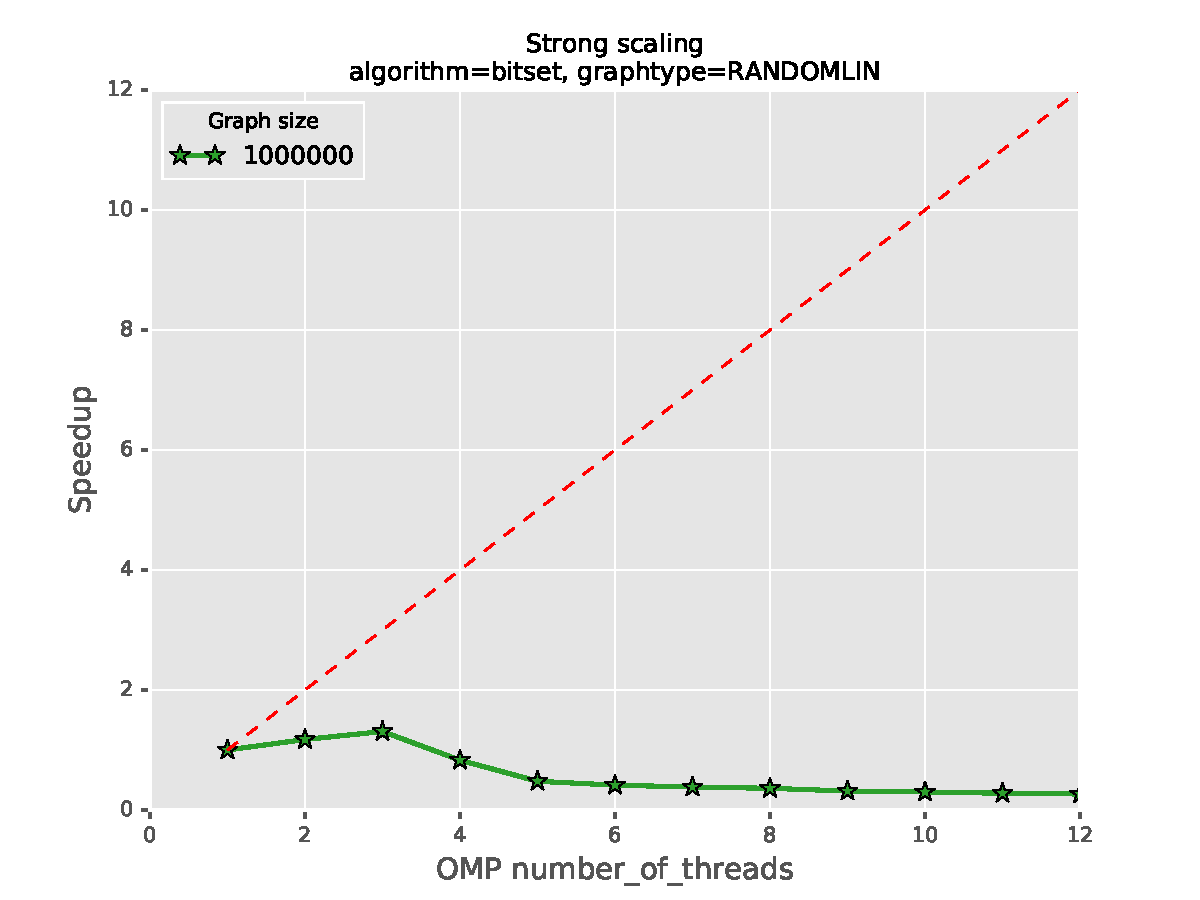
\includegraphics[width=\textwidth]{img/strongscaling_bitset_gtRANDOMLIN30_opt0.pdf}
    \end{center}
  \end{figure}  
\end{columns}

\begin{table}
\tiny
\begin{tabular}{lp{1cm}|p{1cm}}
 {\bfseries Absolute runtimes on 1 core}  & optimistic  & conventional \\
                                          & 3.51 s      & 3.52 s
\end{tabular}
\end{table}

\end{frame}

\begin{frame}
 \frametitle{Absolute runtime composition}
 \begin{columns}[T]
 \column{0.5\textwidth}
  \bfseries{Local lists}
  \begin{figure}[!ht]
    \begin{center}
      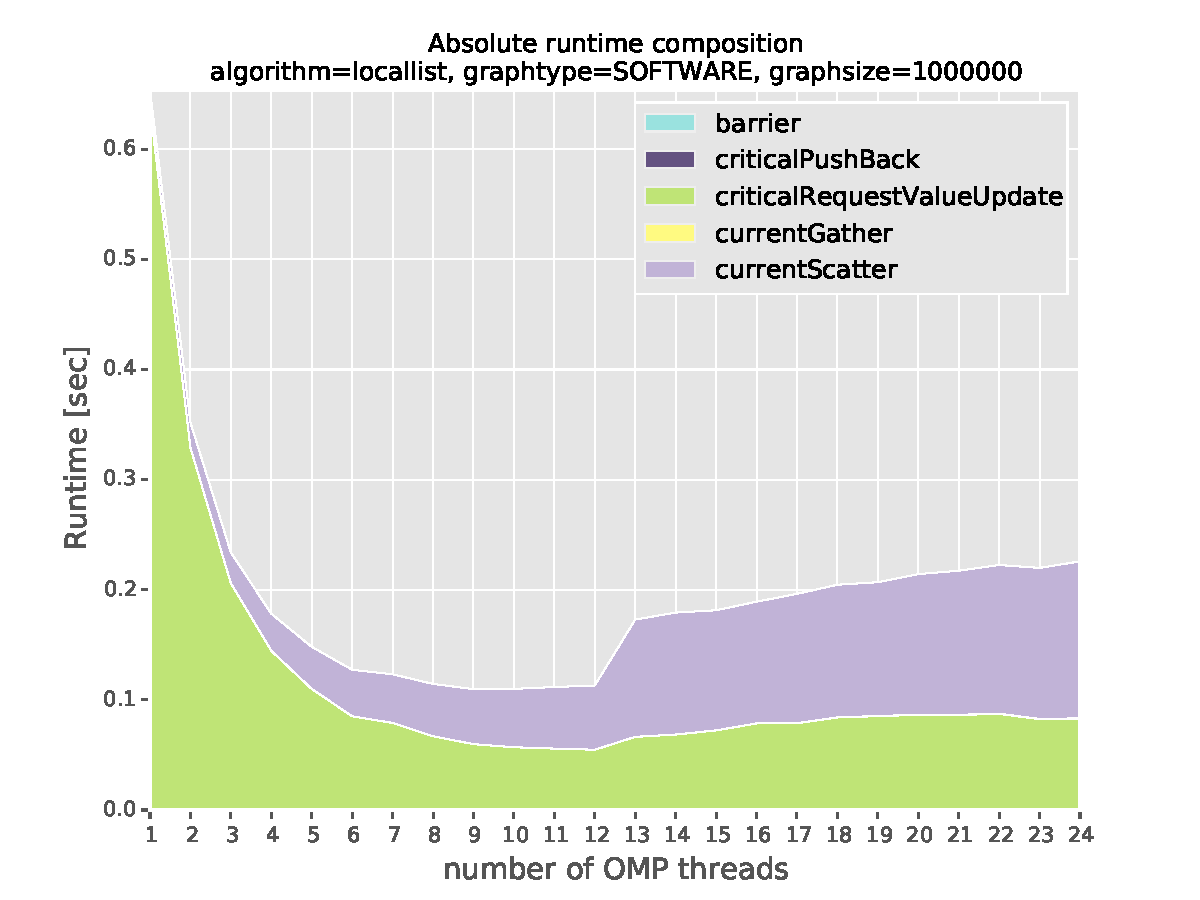
\includegraphics[width=\textwidth]{img/timeabs_locallist_gtSOFTWARE_s1000000_opt0.pdf}
    \end{center}
  \end{figure}

 \column{0.5\textwidth}
  \bfseries{Bool array}
  \begin{figure}[!ht]
    \begin{center}
      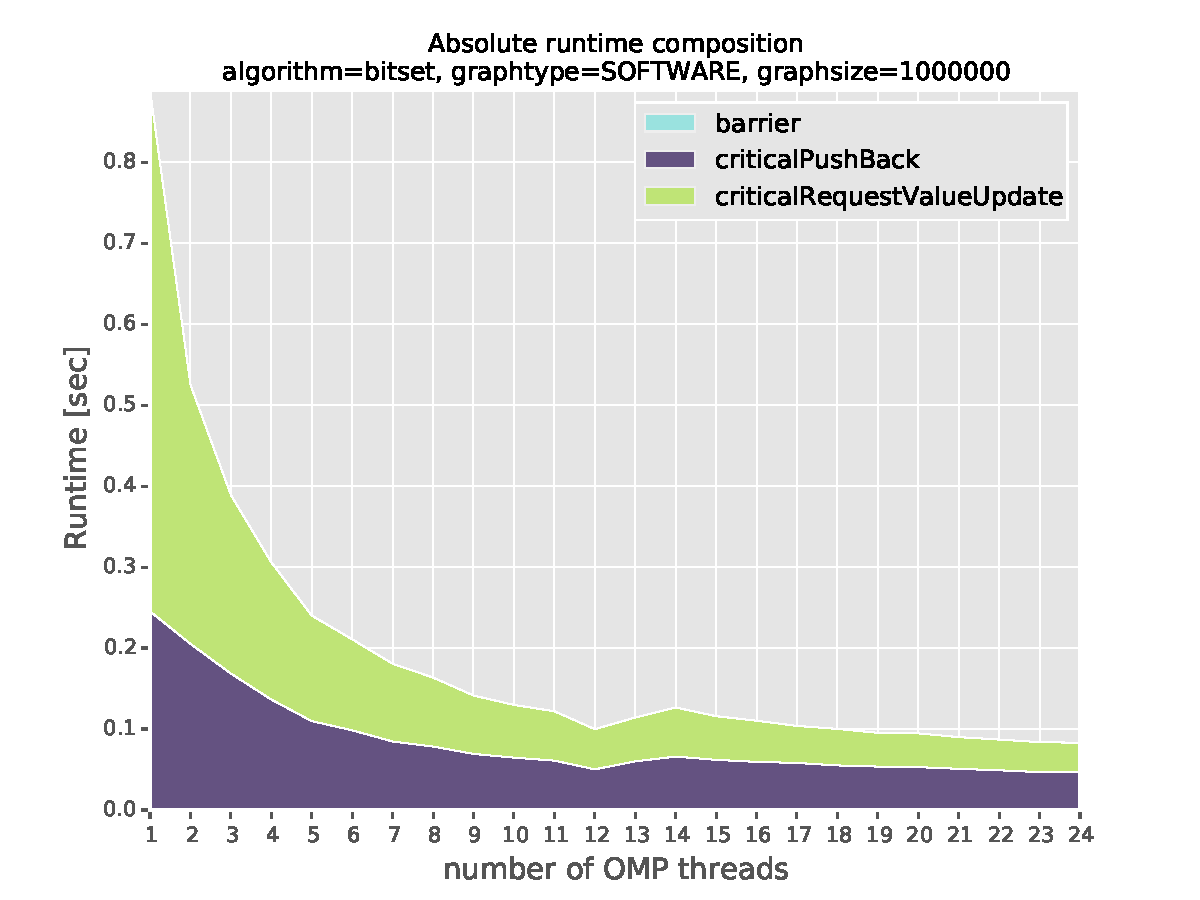
\includegraphics[width=\textwidth]{img/timeabs_bitset_gtSOFTWARE_s1000000_opt1.pdf}
    \end{center}
  \end{figure}
\end{columns}
 
\end{frame}



\begin{frame}
 \frametitle{Remaining issues}
 \begin{itemize}
	 \item Pinpoint the reasons for bad scaling
	 \item Work stealing could help to improve local list approach
 \end{itemize}
\end{frame}



\begin{frame}
\frametitle{References}
\footnotesize{
\begin{thebibliography}{999} % Beamer does not support BibTeX so references must be inserted manually as below

	\bibitem[M. C. Er, 1983] {syncval} M. C. Er.
		\newblock A Parallel Computation Approach to Topological Sorting
		\newblock \emph{The Computer Journal}, Vol 28, 1983, Wiley Heyden Ltd	
	
	\bibitem[Musco, V. et al., 2014] {softwaregraph} V. Musco, M. Monperrus, P. Preux
		\newblock A Generative Model of Software Dependency Graphs to Better Understand Software Evolution
		\newblock \emph{arXiv} 1410.7921

\end{thebibliography}
}
\end{frame}


\end{document} 
